\section{Experimental Higgs boson highlights}
%%%%%%%%%%%%%%%%%%%%%%%%%%%%%%%%%%%%%%%%%%%%%%%%%%%%%%%%%%%%%%%%%%%%%%
\label{sec:HiggsExp}

The discovery of the new boson has been followed by a comprehensive set of measurements aimed at establishing the properties of the particle. Latest results reported by both the ATLAS and CMS experiments are consistent with the SM expectations for the Higgs boson. The properties that have been measured mainly are:

\begin{itemize}
\item the signal strength modifier $\mu = \sigma/\sigma_\mathrm{SM}$, where $\sigma$ is the observed production cross section and $\sigma_\mathrm{SM}$ is the value predicted by the SM for a given mass hypothesis;

\item the couplings to bosons and fermions;

\item the spin and parity;

\item the total decay width of the resonance.
\end{itemize}

Moreover, the combination of the results of the two experiments has recently been performed concerning the mass of the new boson, which is found to be $m_\mathrm{H} = 125.09 \pm 0.21 ~\text{(stat.)} \pm 0.11~\text{(syst.)}$\GeV~\cite{Aad:2015zhl}.

The CMS experiment has investigated the Higgs boson decays to ZZ, \WW, $\gamma\gamma$, $\tau^+\tau^-$ and $\mathrm{b \bar b}$ using 2011 and 2012 data, and is now looking at the same channels using new data collected at a centre-of-mass energy of 13\TeV. The 8\TeV CMS results of all channels have been combined and the best-fit signal strength corresponding to the measured mass is found to be $\mu = 1.00 \pm 0.09~\text{(stat.)} ^{+0.08}_{-0.07}~\text{(theo.)} \pm  0.07~\text{(syst.)}$~\cite{Khachatryan:2014jba}, in good agreement with the SM expectation of $\mu=1$.
The signal strengths modifiers obtained in different sub-combinations of channels for $m_\mathrm{H}=125$\GeV are shown in Fig.~\ref{fig:signal_strengths}, grouped by production mode tag and decay channel.

\begin{figure}[htb]
\centering
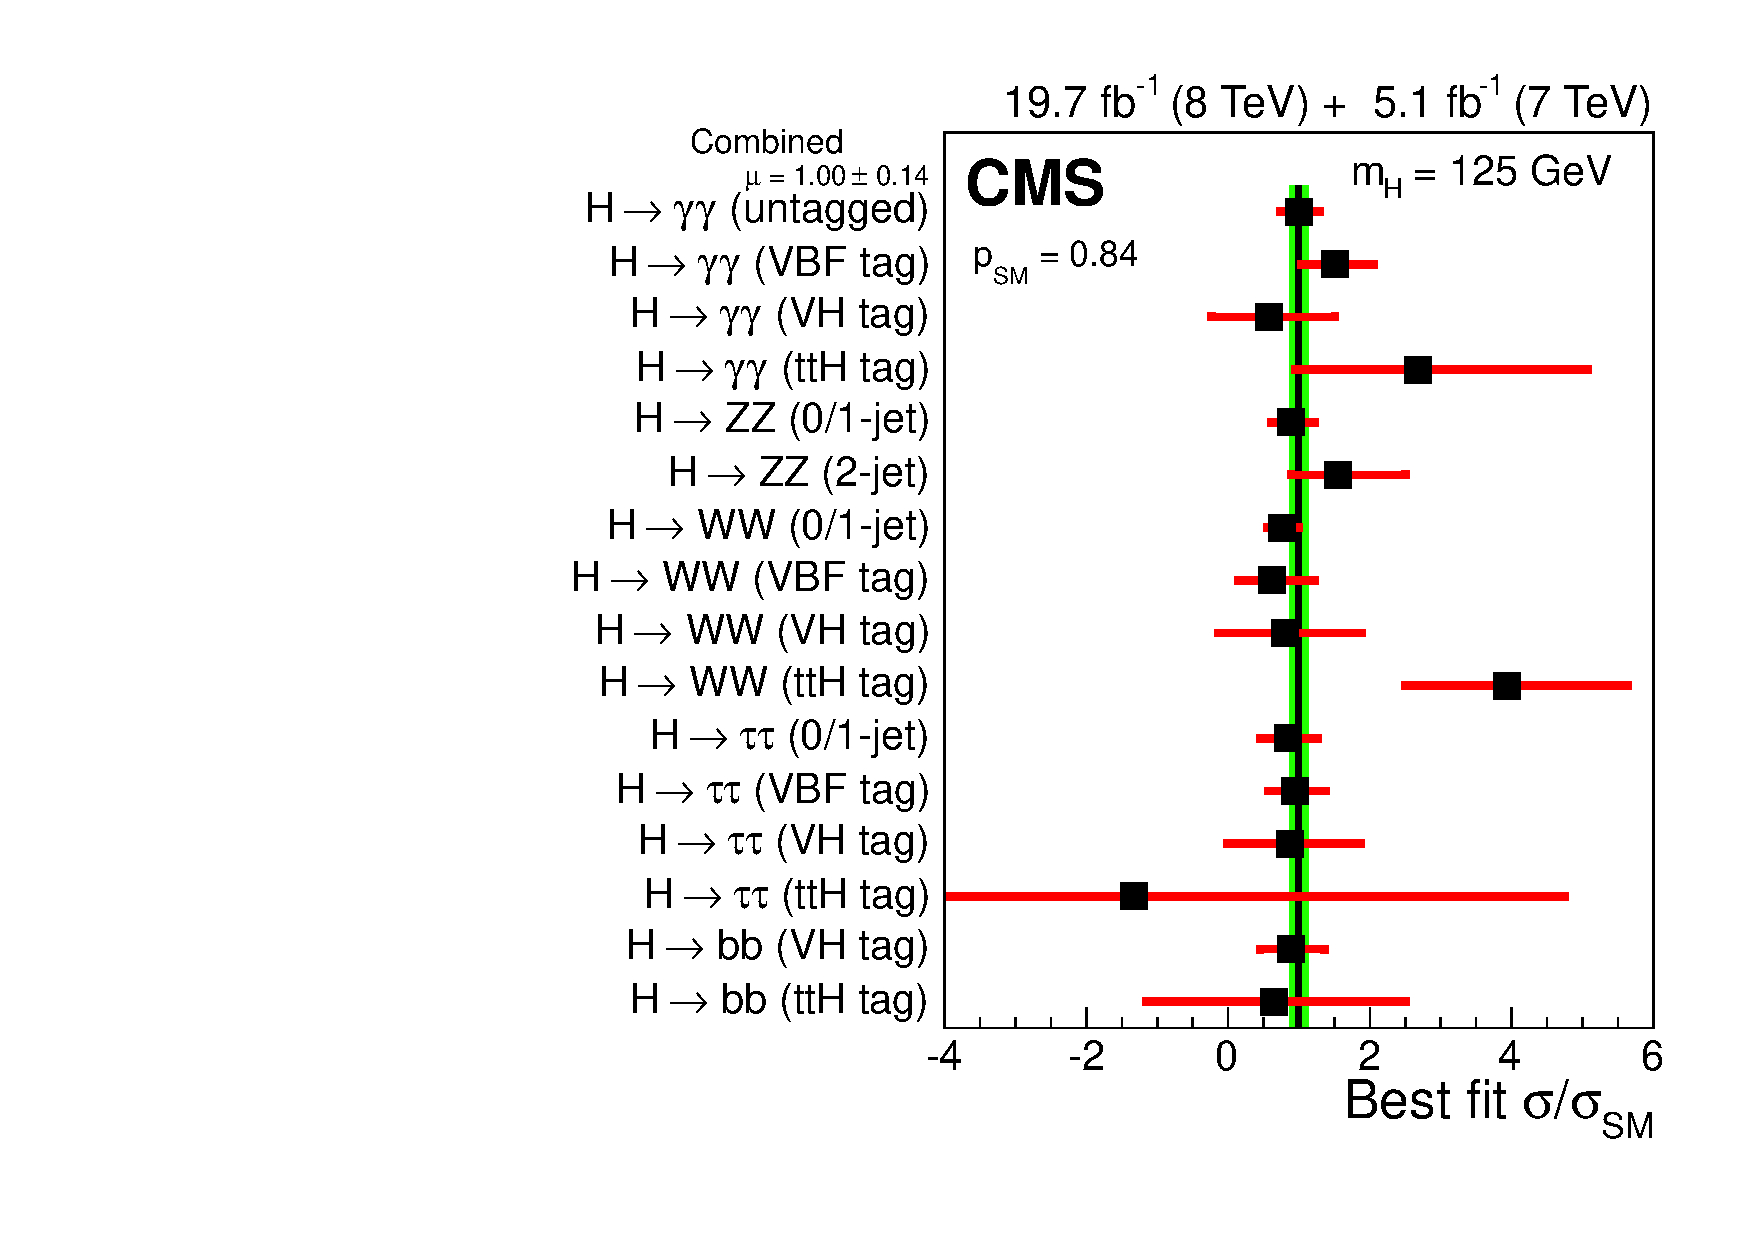
\includegraphics[width=0.5\textwidth]{images/signal_strengths.pdf}
\caption{Values of the best-fit $\mu$ for the combination of all analyses (solid vertical line) and separate combinations grouped by production mode tag and decay channel. The vertical band represents the total uncertainty on the combination while the horizontal red bars correspond to uncertainties on the individual channels.}\label{fig:signal_strengths}
\end{figure}

The combination of all measurements in all decay channels is used to extract ratios between the observed coupling strengths and those predicted by the SM. The formalism used to test for deviations from the SM expectations has been established by the LHC Higgs Cross Section Working Group in Ref.~\cite{Heinemeyer:2013tqa}. This formalism makes some assumptions, in particular that the observed state has $J^P =0^+$ and that the narrow width approximation holds, leading to a factorization of the coupling strengths for production and decay modes. As an example, Higgs boson events produced via ggH and decaying to \WW, i.e. $\mathrm{gg\to H\to W^+W^-}$, can be used to measure the Higgs boson coupling to W bosons and fermions (mainly top quarks that are present in the gluon fusion loop). The combination of ATLAS and CMS results using data collected at 7 and 8\TeV is used to test the Higgs boson coupling to fermions $k_F$ and bosons $k_V$~\cite{Khachatryan:2016vau}. The contours at 68\% CL in the $(k_F^f, k_V^f)$ plane (where the $f$ refers to the generic decay channel $\mathrm{H\to f}$) for the combination of ATLAS and CMS results and for the individual channels are shown in Fig.~\ref{fig:couplings}.

\begin{figure}[htb]
\centering
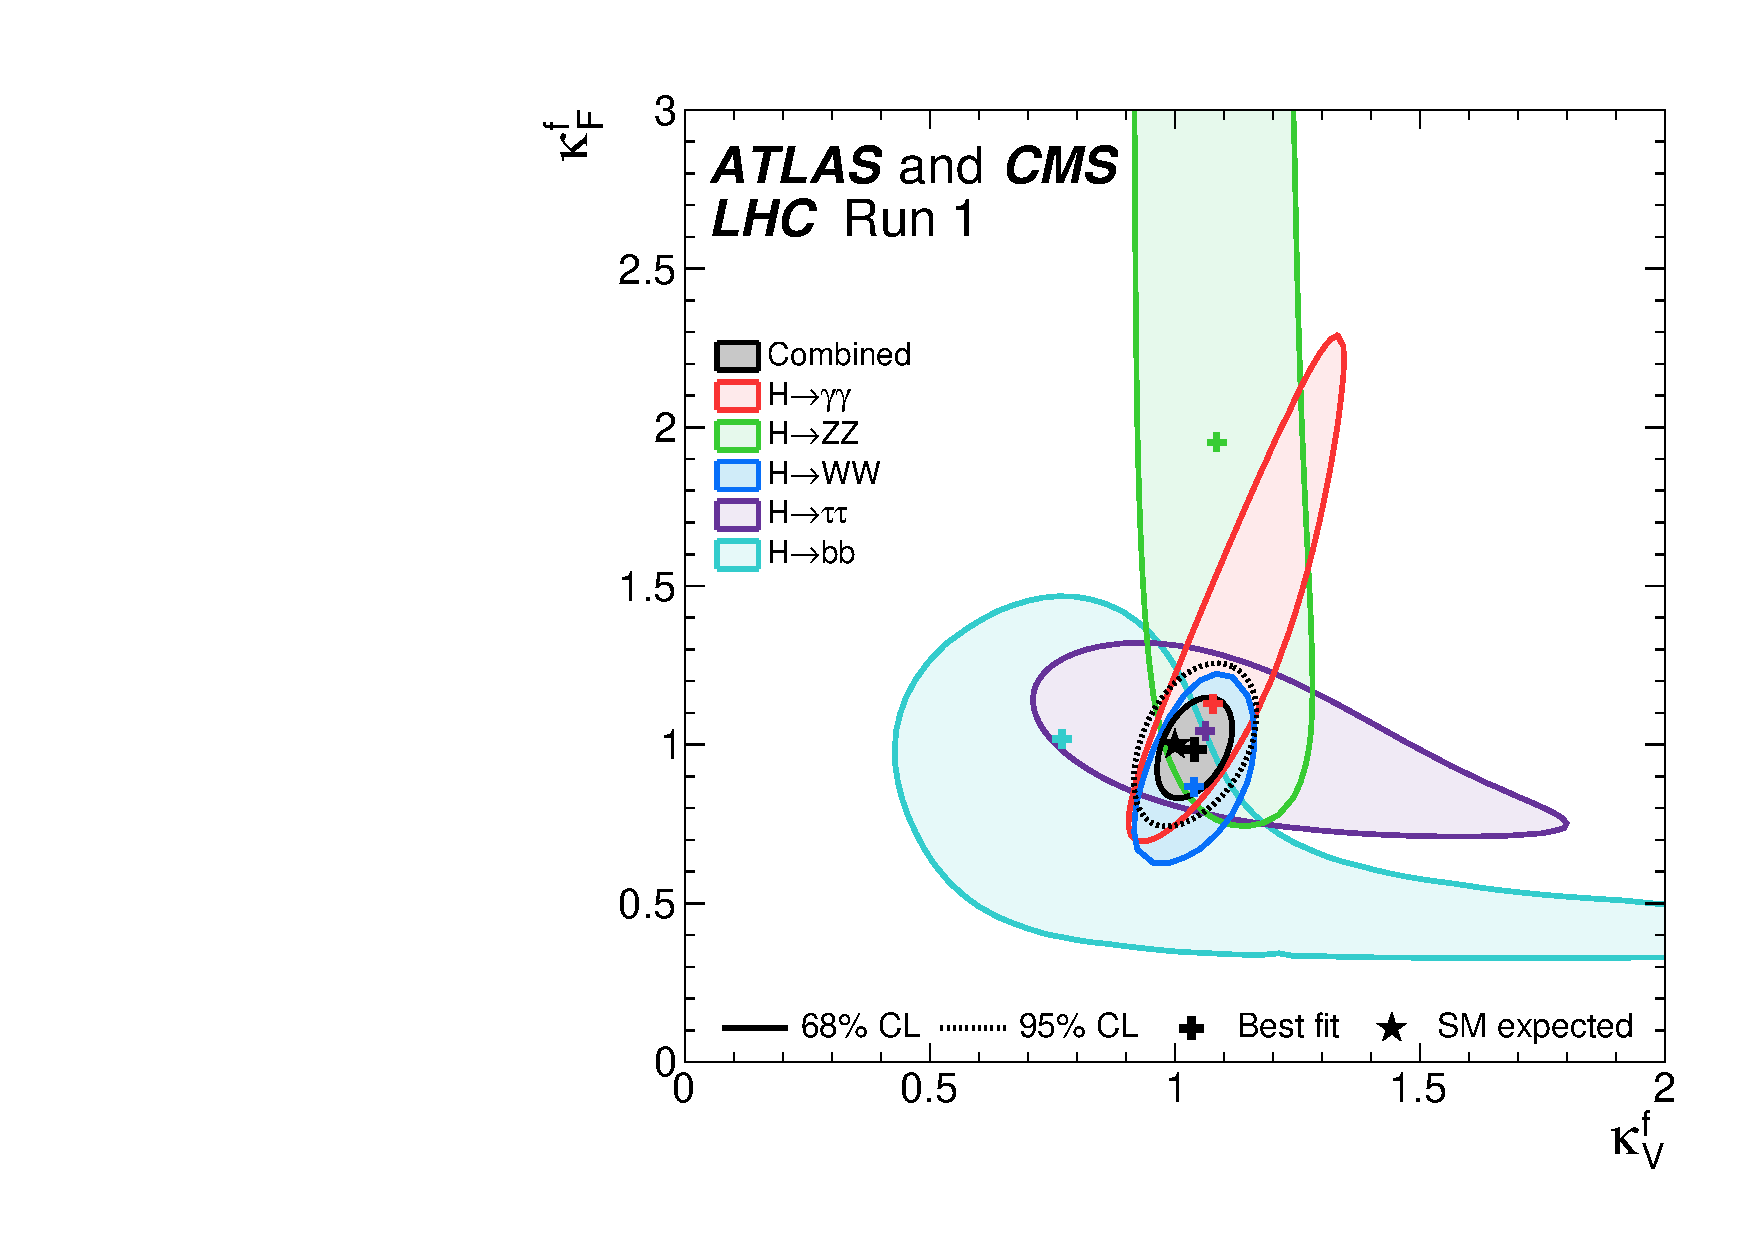
\includegraphics[width=0.5\textwidth]{images/couplings.pdf}
\caption{Contours at 68\% CL in the $(k_F^f, k_V^f)$ plane for the combination of ATLAS and CMS results and for the individual channels.}\label{fig:couplings}
\end{figure}

The combined result is in agreement with the SM expectation and the final confidence interval is driven by the \hww channel, which provides the most precise determination of $k_F^f$ and $k_V^f$ because it is the only channel that allows significant constraints on both parameters through the measurements of the ggH and VBF production processes.

About the spin and parity properties, the results of the $\mathrm{H\to \gamma\gamma}$, $\mathrm{H\to ZZ\to 4\ell}$ and \hwwllnn channels confirmed the hypothesis of a scalar boson ($J^P = 0^+$), excluding the other hypotheses with a confidence level of 99\% or higher.

The Higgs boson total decay width ($\Gamma_\mathrm{H}$) is predicted by the SM as a function of its mass, as shown in Fig.~\ref{fig:width}. At $m_\mathrm{H}=125$\GeV the Higgs boson is predicted to be a narrow resonance, with a total decay width of the order of 4.1\MeV. Direct measurements of the decay width have been performed in the $\mathrm{H\to ZZ\to 4\ell}$ and $\mathrm{H\to\gamma\gamma}$ channels, but the results are limited by the experimental resolution, which is about three orders of magnitude larger than the expected value, thus not allowing to provide significant constraints. The sizeable off-shell production of the Higgs boson can also be used to constrain its natural width. In fact, a measurement of the relative off-shell and on-shell production provides direct information on $\Gamma_\mathrm{H}$~\cite{Caola:2013yja}, under the assumption that the Higgs boson off- and on-shell production mechanisms are the same as in the SM and the ratio of couplings governing the two remains unchanged with respect to the SM predictions. Using this technique and combining the CMS results of the $\mathrm{H\to ZZ\to 4\ell}$ and \hwwllnn channels, the upper limit at 95\% CL on the Higgs boson total decay width is found to be $\Gamma_\mathrm{H}^\mathrm{obs} < 13$\MeV~\cite{Khachatryan:2016ctc}, which represents a far better constraint with respect to direct measurements.

\begin{figure}[htb]
\centering
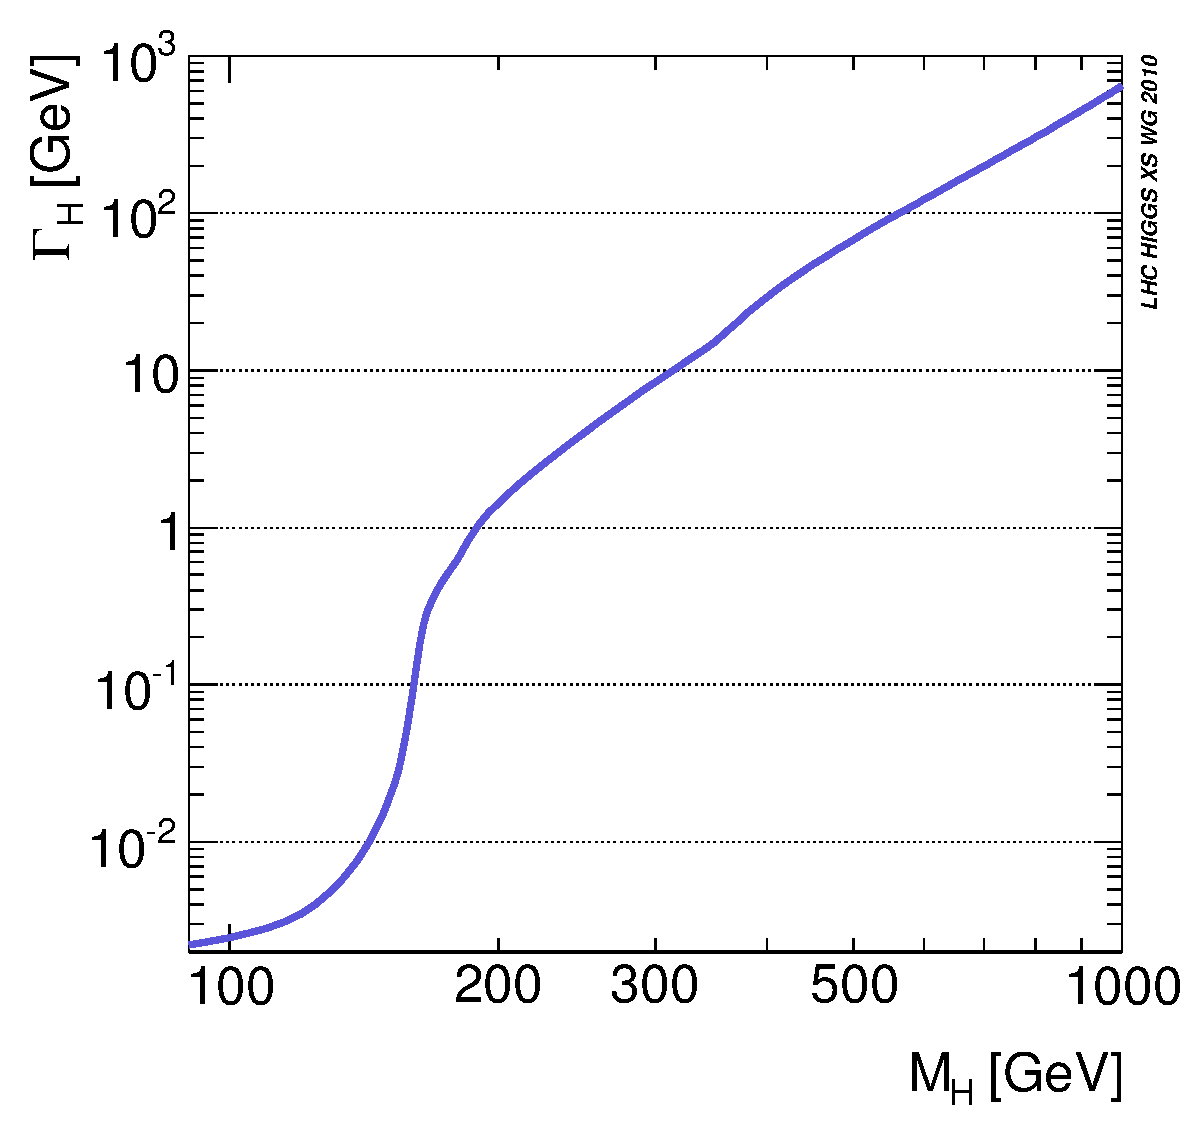
\includegraphics[width=0.45\textwidth]{images/width.pdf}
\caption{Total decay width of the SM Higgs boson as a function of $m_\mathrm{H}$.}\label{fig:width}
\end{figure}

Differential cross section measurements have also been performed by both experiments in the bosonic channels, $\gamma\gamma$, ZZ and $\mathrm{W^+W^-}$ (the latter is presented in Chapter~\ref{chap4} of this work), showing agreement with the SM-based theoretical predictions.
